\newpage
\section{Exercícios Práticos}

Esta seção apresenta exercícios para consolidar os conceitos abordados ao longo da apostila. Os exercícios estão divididos em níveis de dificuldade e incluem um mini-projeto colaborativo, permitindo que você pratique desde os comandos básicos até situações reais de trabalho em equipe com Git.

Para todos os exercícios dessa seção, o ambiente integrado de desenvolvimento Visual Studio Code será utilizado.

\subsection{Nível Iniciante}

\subsubsection{Criar um Repositório Local}
\begin{itemize}
    \item Crie uma pasta chamada \texttt{meu\_projeto\_git} em seu computador.

    \begin{figure}[H]
        \centering
        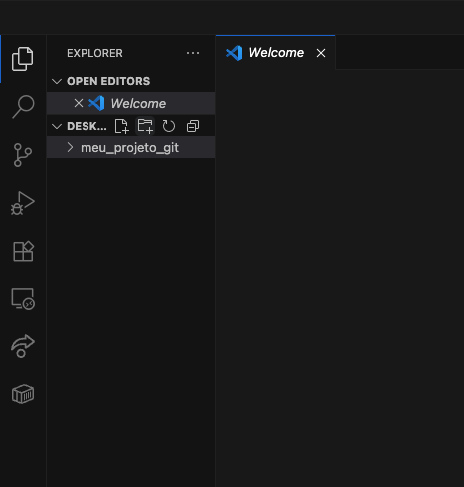
\includegraphics[width=0.6\textwidth]{imgs/tutorial_github/ex01_01.png}
        \label{fig:ex01_01}
        \caption{Solução do exercício 01: Criando a pasta meu\_projeto\_git no VS Code.}
    \end{figure}

    \begin{figure}[H]
        \centering
        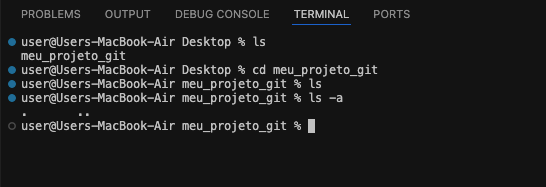
\includegraphics[width=0.6\textwidth]{imgs/tutorial_github/ex01_01_1.png}
        \label{fig:ex01_01_01}
        \caption{Solução do exercício 01: Utilizando o terminal do VS Code e alguns comandos para entrar na pasta meu\_projeto\_git e verificar os arquivos da pasta.}
    \end{figure}


    \item Inicialize um repositório Git na pasta:
    \begin{lstlisting}[style=shellstyle]
git init
    \end{lstlisting}


    \begin{figure}[H]
        \centering
        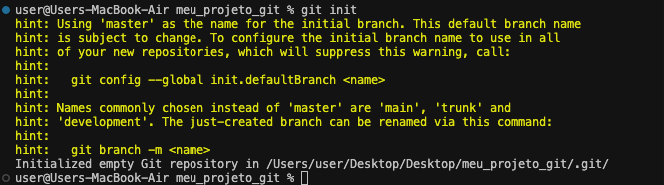
\includegraphics[width=0.6\textwidth]{imgs/tutorial_github/ex01_02.png}
        \label{fig:ex01_02}
        \caption{Solução do exercício 01: Inicializando o repositório git.}
    \end{figure}
    
    \item Verifique o status do repositório:
    \begin{lstlisting}[style=shellstyle]
git status
    \end{lstlisting}

    \begin{figure}[H]
        \centering
        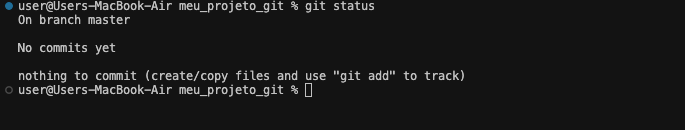
\includegraphics[width=0.6\textwidth]{imgs/tutorial_github/ex01_03.png}
        \label{fig:ex01_03}
        \caption{Solução do exercício 01: Verificando o status do repositório.}
    \end{figure}
    
\end{itemize}



\subsubsection{Rastrear Arquivos e Fazer Commits}
\begin{itemize}
    \item Crie um arquivo chamado \texttt{README.md} e escreva uma breve descrição do projeto.

       \begin{figure}[H]
        \centering
        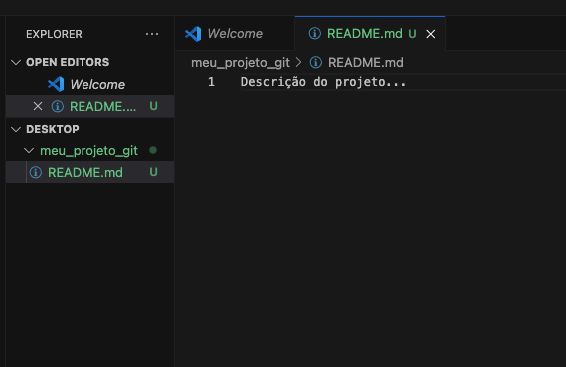
\includegraphics[width=0.6\textwidth]{imgs/tutorial_github/ex02_01.png}
        \label{fig:ex02_01}
        \caption{Solução do exercício 02: Criando o arquivo README.md.}
    \end{figure}

    \begin{figure}[H]
        \centering
        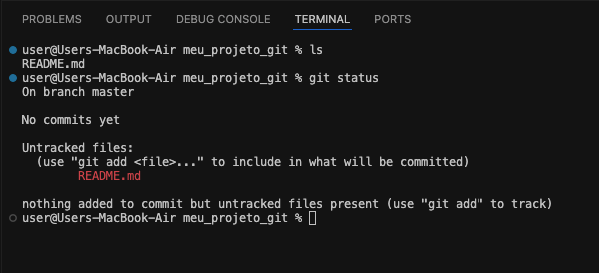
\includegraphics[width=0.6\textwidth]{imgs/tutorial_github/ex02_01_01.png}
        \label{fig:ex02_01_01}
        \caption{Solução do exercício 02: Git status retorna que README.md é um novo arquivo que precisa ser adicionado ao repositório git.}
    \end{figure}
    
    \item Adicione o arquivo ao staging area:
    \begin{lstlisting}[style=shellstyle]
git add README.md
    \end{lstlisting}
    \item Faça um commit com uma mensagem clara:
    \begin{lstlisting}[style=shellstyle]
git commit -m "Adiciona README inicial"
    \end{lstlisting}

    \begin{figure}[H]
        \centering
        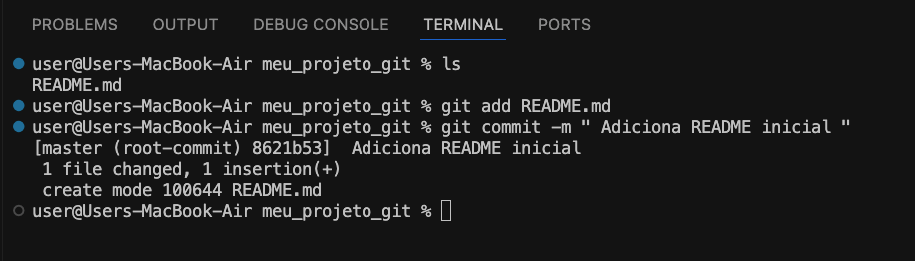
\includegraphics[width=0.6\textwidth]{imgs/tutorial_github/ex02_02.png}
        \label{fig:ex02_02}
        \caption{Solução do exercício 02: Adicionando README.md e fazendo o commit.}
    \end{figure}
    
    \item Crie mais um arquivo (ex: \texttt{codigo.m}) e repita o processo:
    \begin{lstlisting}[style=shellstyle]
git add codigo.m
git commit -m "Adiciona código MATLAB inicial"
    \end{lstlisting}

    \begin{figure}[H]
        \centering
        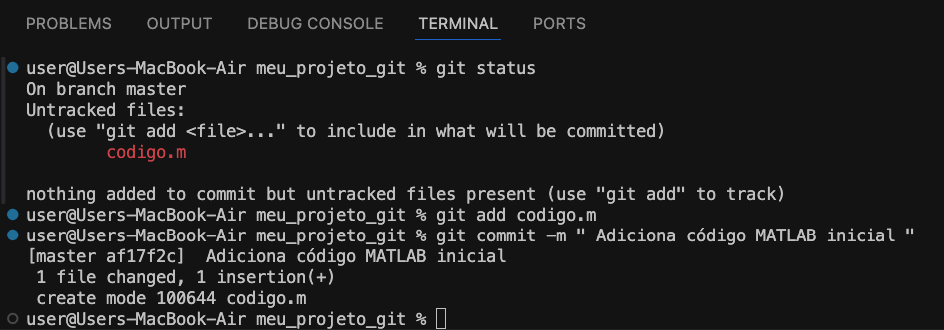
\includegraphics[width=0.6\textwidth]{imgs/tutorial_github/ex02_03.png}
        \label{fig:ex02_03}
        \caption{Solução do exercício 02: Adicionando codigo.m e fazendo o commit.}
    \end{figure}
    
\end{itemize}

\subsubsection{Enviar para um Repositório Remoto}
\begin{itemize}
    \item Crie um repositório remoto no GitHub ou GitLab.

    \begin{figure}[H]
        \centering
        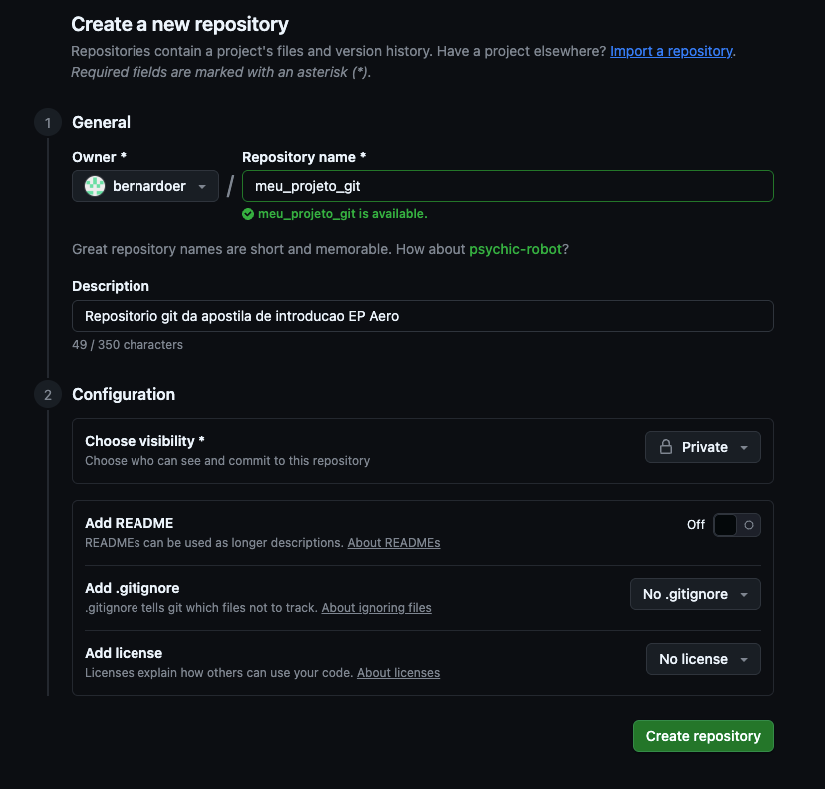
\includegraphics[width=0.6\textwidth]{imgs/tutorial_github/ex03_01.png}
        \label{fig:ex03_01}
        \caption{Solução do exercício 03: Criando o repositório no GitHub.}
    \end{figure}
    
    \item Conecte o repositório local ao remoto:
    \begin{lstlisting}[style=shellstyle]
git remote add origin <URL-do-repositório>
    \end{lstlisting}

    
    \item Envie seus commits para o remoto:
    \begin{lstlisting}[style=shellstyle]
git push origin main
    \end{lstlisting}

    \begin{figure}[H]
        \centering
        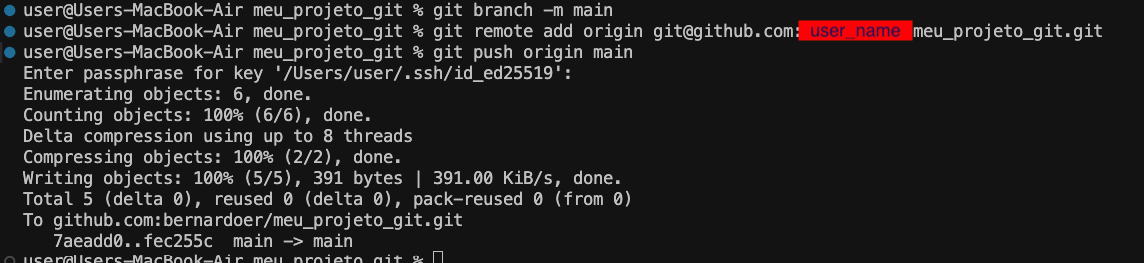
\includegraphics[width=0.6\textwidth]{imgs/tutorial_github/ex03_03.png}
        \label{fig:ex03_02}
        \caption{Solução do exercício 03: Adicionando a branch master no repositório GitHub.}
    \end{figure}
\end{itemize}

\subsection{Nível Intermediário}

\subsubsection{Criar e Mesclar Branches}
\begin{itemize}
    \item Crie um branch chamado \texttt{feature/descricao}:
    \begin{lstlisting}[style=shellstyle]
git checkout -b feature/descricao
    \end{lstlisting}
    \item No novo branch, edite o \texttt{README.md} adicionando mais detalhes sobre o projeto.
    \item Adicione e faça commit das alterações:
    \begin{lstlisting}[style=shellstyle]
git add README.md
git commit -m "Adiciona detalhes ao README"
    \end{lstlisting}
    \item Retorne ao branch principal:
    \begin{lstlisting}[style=shellstyle]
git checkout main
    \end{lstlisting}
    \item Mescle o branch de funcionalidade:
    \begin{lstlisting}[style=shellstyle]
git merge feature/descricao
    \end{lstlisting}
\end{itemize}

 \begin{figure}[H]
        \centering
        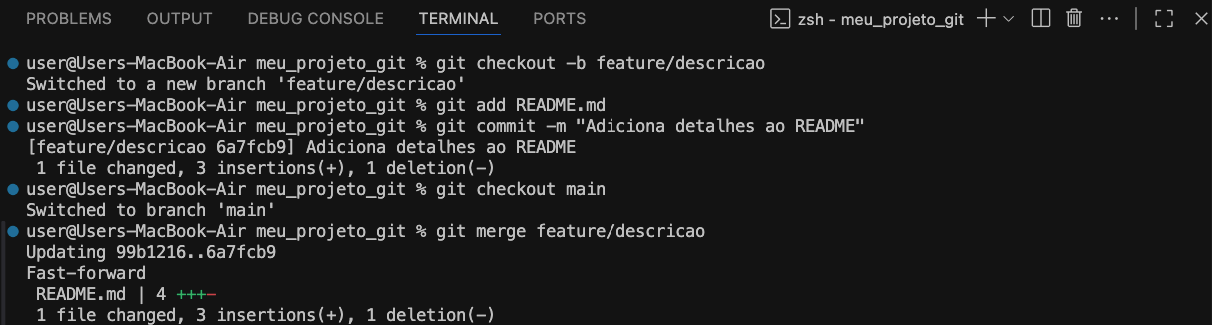
\includegraphics[width=0.6\textwidth]{imgs/tutorial_github/ex04_01.png}
        \label{fig:ex04_01}
        \caption{Solução do exercício 04: Criando feature branch para editar o projeto.}
    \end{figure}

\subsubsection{Resolver Conflitos de Merge}
\begin{itemize}
    \item Simule um conflito editando a mesma linha do \texttt{README.md} em dois branches diferentes.
    \item Tente fazer o merge e, ao encontrar um conflito, edite o arquivo manualmente para resolver.
    \item Após resolver, adicione e faça commit:
    \begin{lstlisting}[style=shellstyle]
git add README.md
git commit -m "Resolve conflito de merge no README"
    \end{lstlisting}
\end{itemize}

\subsubsection{Utilizar Efetivamente o .gitignore}
\begin{itemize}
    \item Crie arquivos temporários (\texttt{.log}, \texttt{.tmp}) na pasta do projeto.
    \item Crie um arquivo \texttt{.gitignore} e adicione regras para ignorar esses arquivos.
    \item Verifique que os arquivos ignorados não aparecem no status:
    \begin{lstlisting}[style=shellstyle]
git status
    \end{lstlisting}
\end{itemize}

\subsection{Mini-Projeto Prático: Gerenciando um Pequeno Projeto de Equipe}

Monte uma equipe de 2 a 4 pessoas e siga os passos abaixo:

\begin{enumerate}
    \item Crie um repositório remoto compartilhado no GitHub ou GitLab.
    \item Cada integrante deve clonar o repositório:
    \begin{lstlisting}[style=shellstyle]
git clone <URL-do-repositório>
    \end{lstlisting}
    \item Divida as tarefas: cada pessoa deve criar um branch para desenvolver uma funcionalidade:
    \begin{lstlisting}[style=shellstyle]
git checkout -b feature/modelo
    \end{lstlisting}
    \item Realize commits frequentes e mensagens claras:
    \begin{lstlisting}[style=shellstyle]
git add <arquivo>
git commit -m "Mensagem clara sobre a alteração"
    \end{lstlisting}
    \item Abra Pull Requests na plataforma para integrar as funcionalidades ao branch principal.
    \item Realize revisões de código e resolva possíveis conflitos de merge.
    \item Ao final, garanta que o projeto esteja organizado, com README atualizado e arquivos desnecessários ignorados pelo \texttt{.gitignore}.
\end{enumerate}

Esses exercícios proporcionam experiência prática com os principais comandos e fluxos de trabalho do Git, preparando você para atuar em projetos reais de engenharia

\subsection{Contribuindo com as apostilas da EP Aero no Github}

Todas as apostilas da EP Aero são disponibilizadas publicamente e de forma gratuita no Github. Os autores da apostila incentivam a contribuição dos leitores para aprimorar o conteúdo, corrigir erros e sugerir melhorias.

Para fazer isso, siga o passo-a-passo a seguir:

\begin{itemize}
        \item Acesse o repositório da apostila no Github: \url{https://github.com/ep-aero-ufsm/apostila-github}
        \item Faça um fork do repositório para sua conta. Para fazer isso, você pode usar a interface web do Github, como mostrado nas figuras \ref{fig:1_fork} e \ref{fig:2_fork}.
\begin{figure}[H]
        \centering
        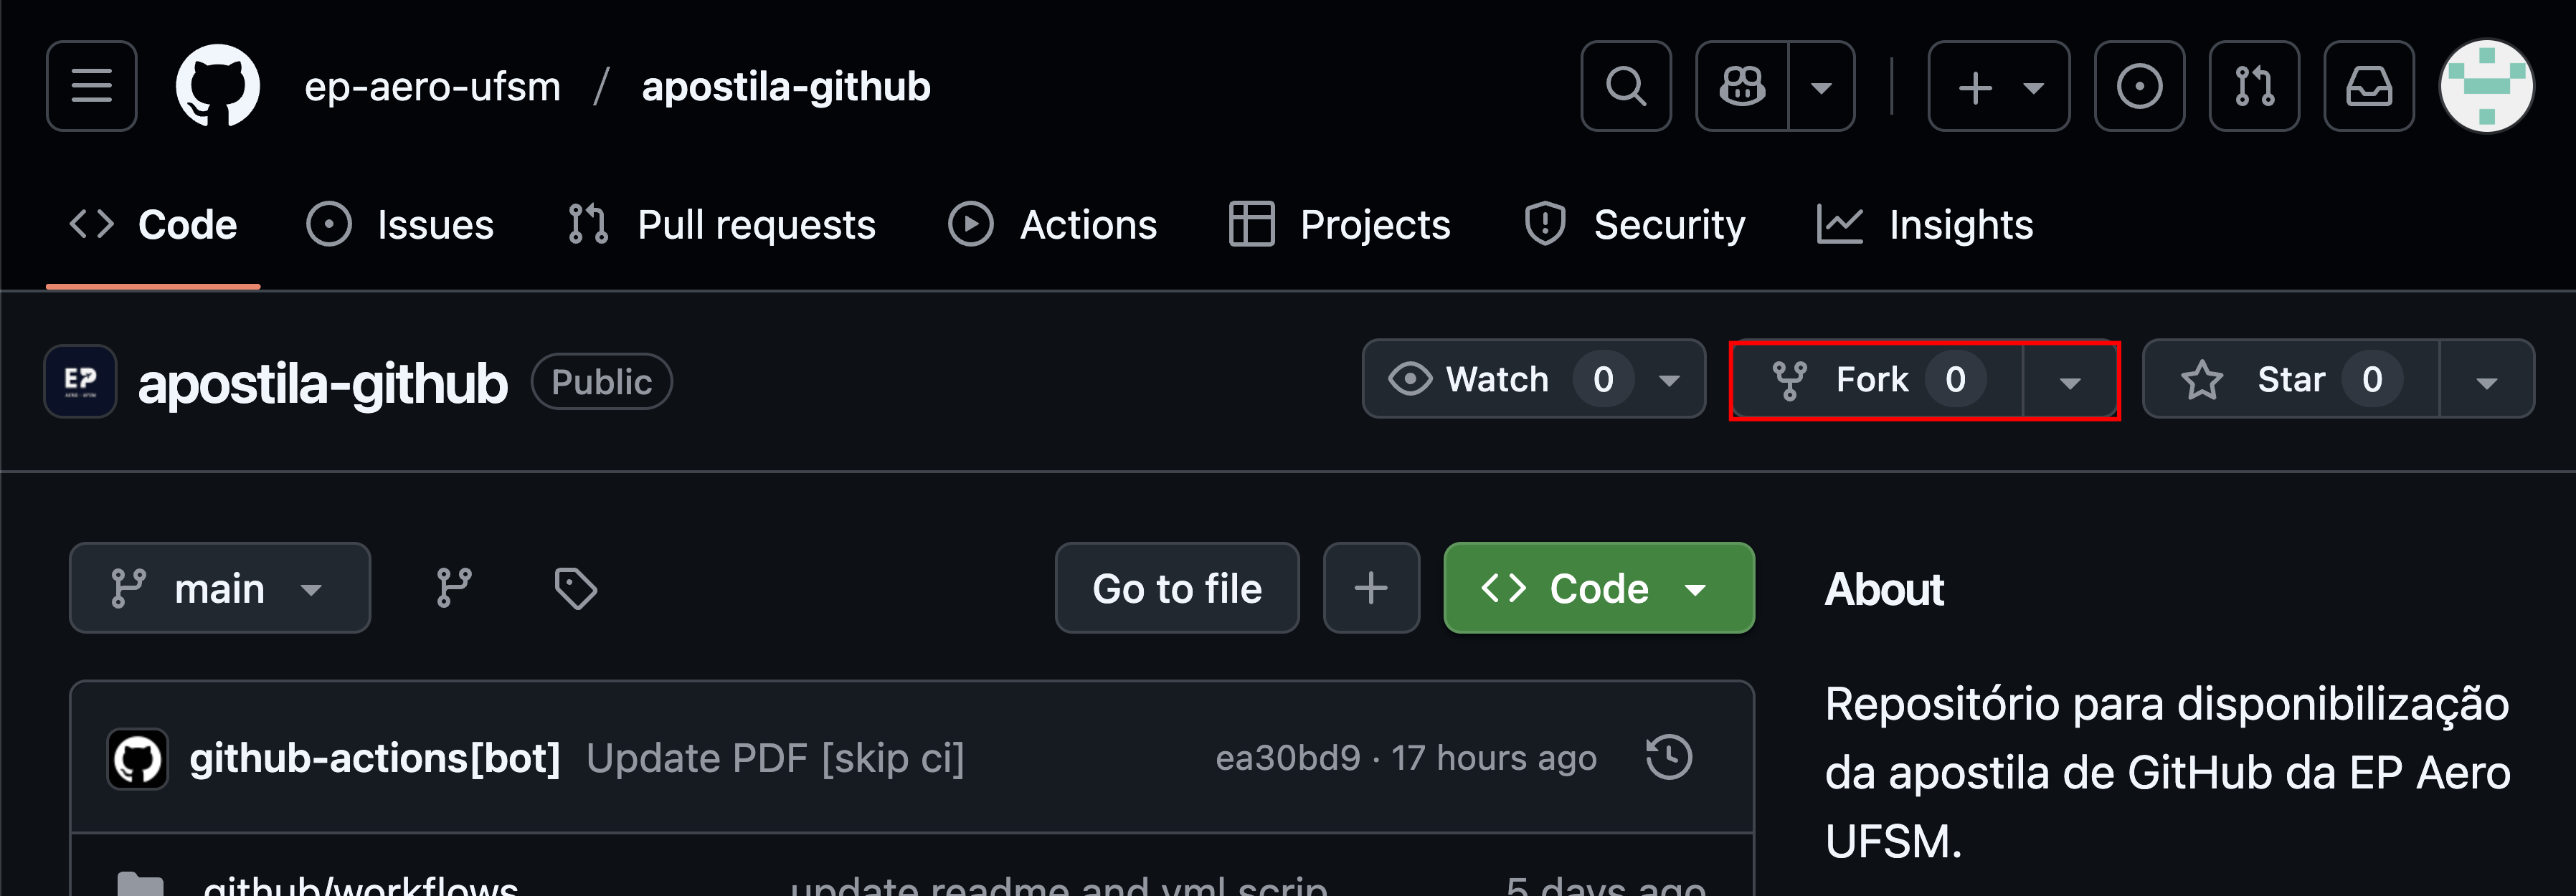
\includegraphics[width=0.6\textwidth]{imgs/tutorial_contribuicao/1_fork.png}
        \caption{Como criar um fork do repositório - etapa 1.}
        \label{fig:1_fork}
    \end{figure}

    \begin{figure}[H]
        \centering
        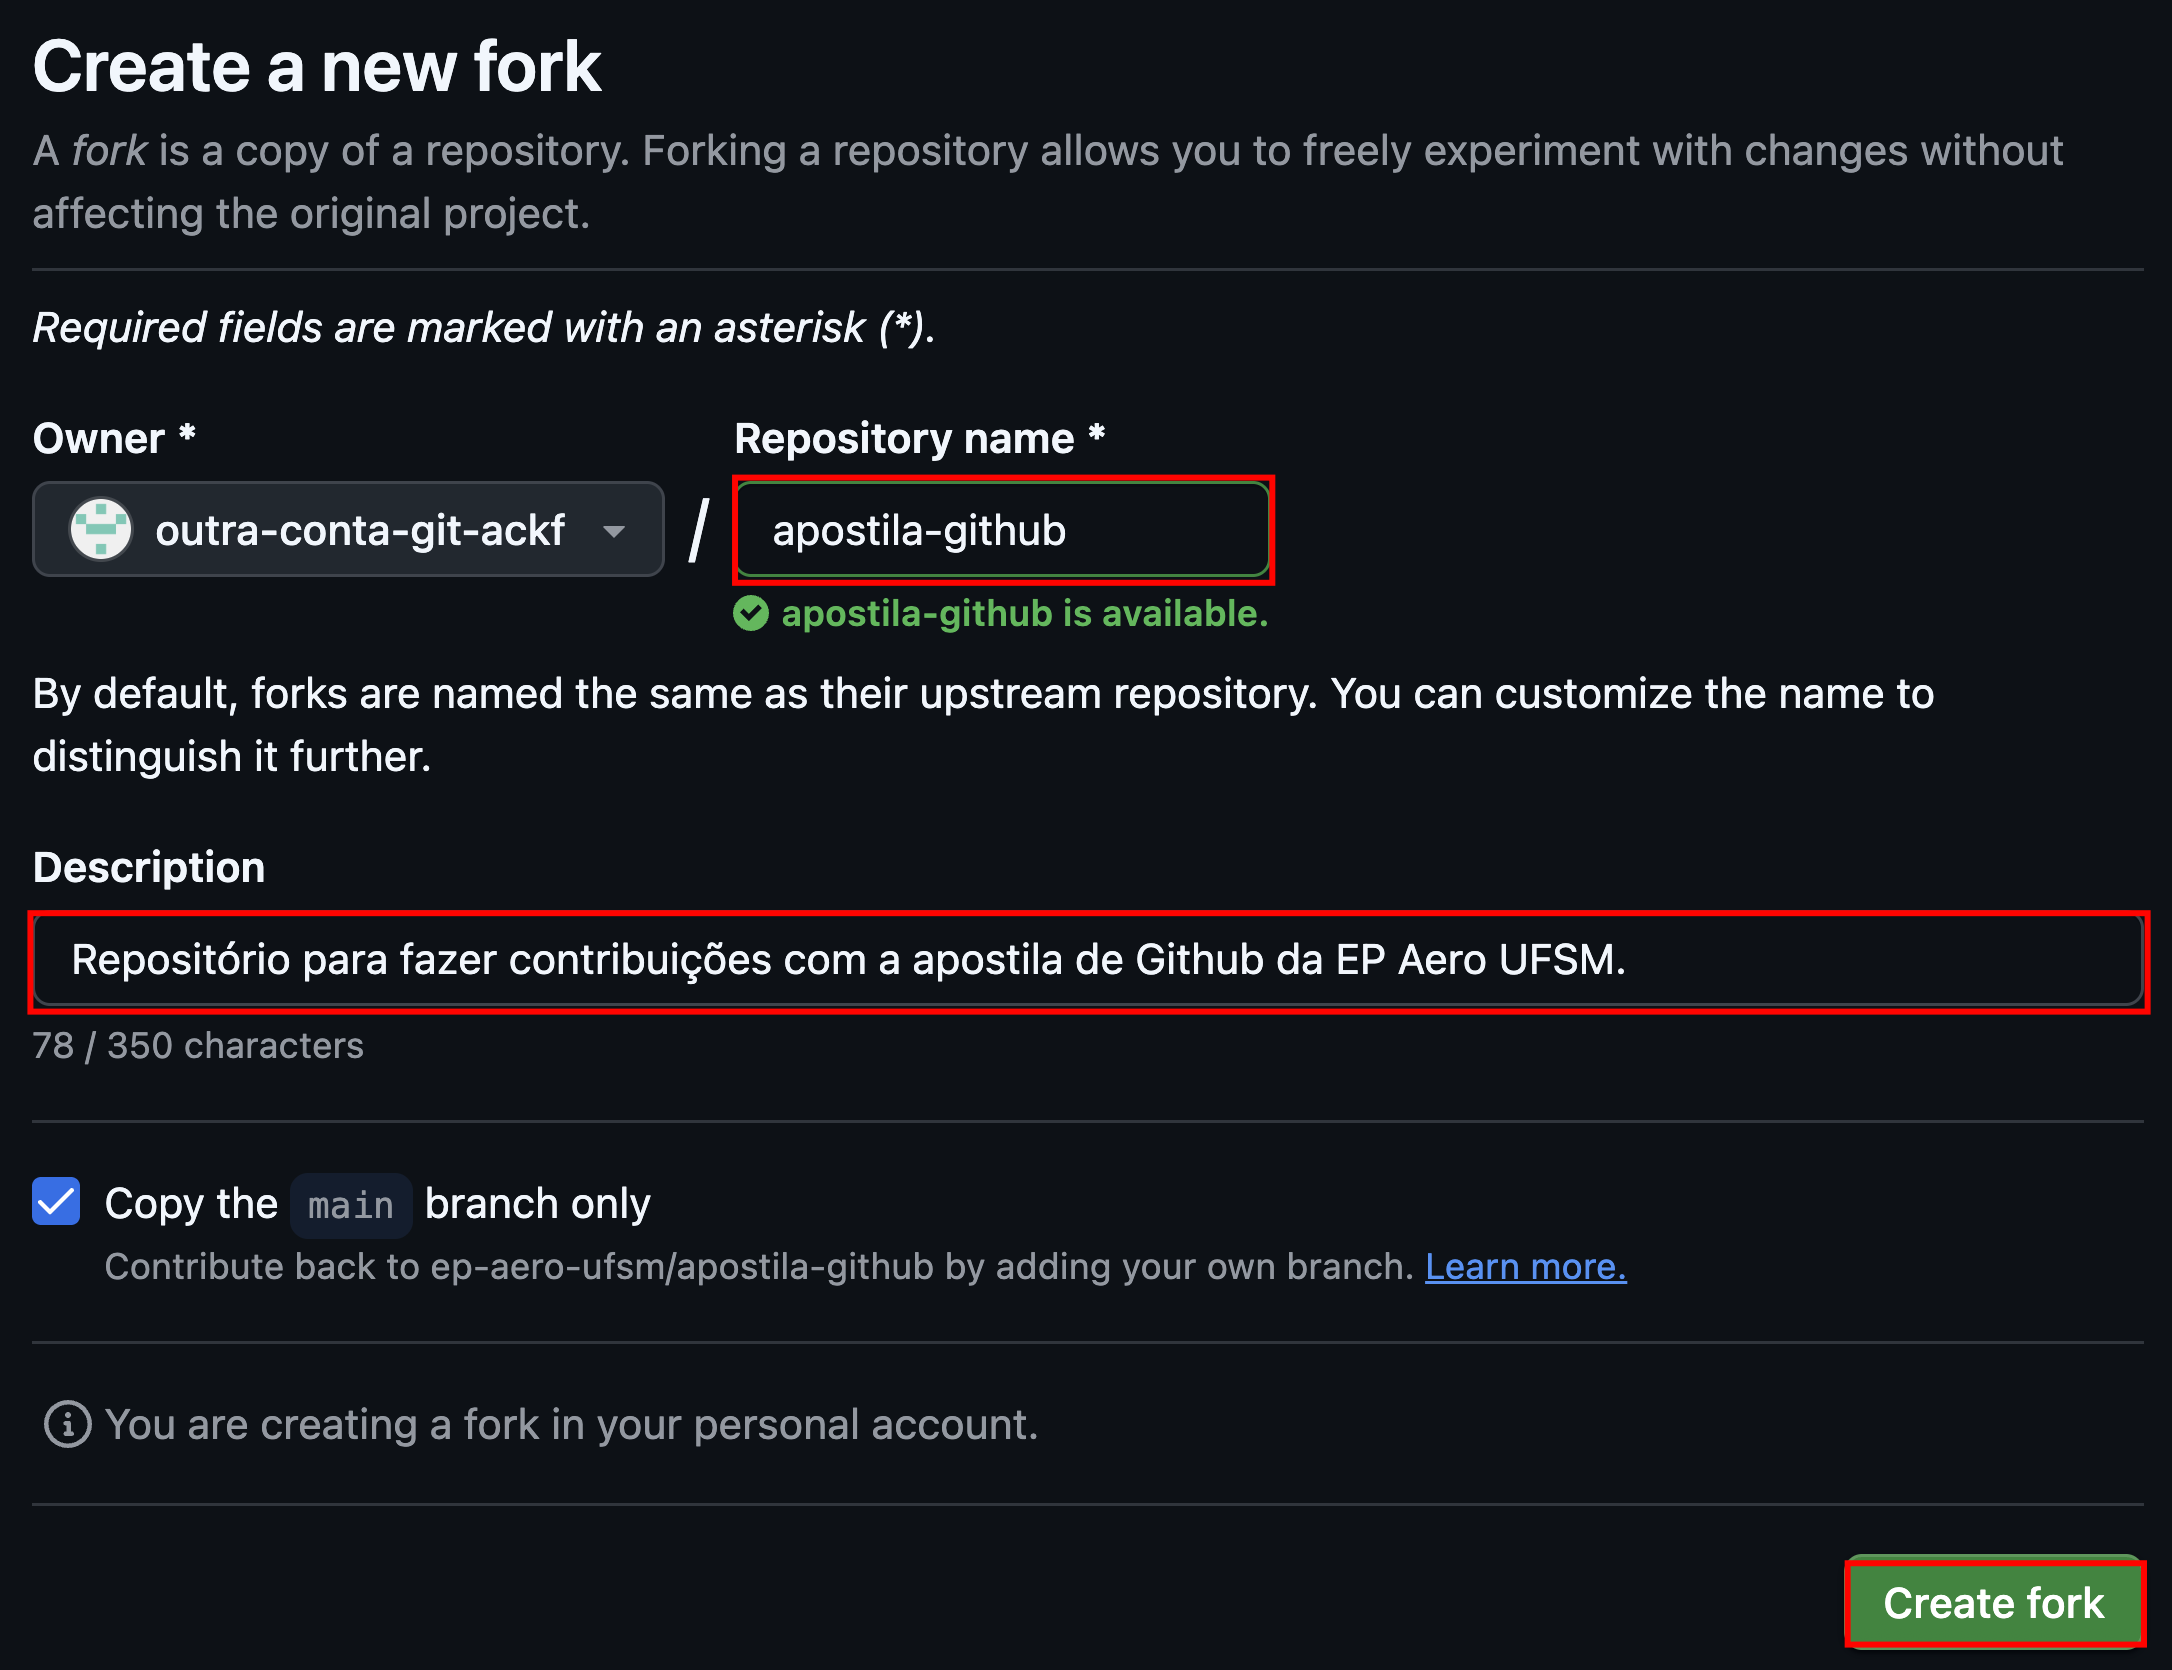
\includegraphics[width=0.6\textwidth]{imgs/tutorial_contribuicao/2_fork.png}
        \caption{Como criar um fork do repositório - etapa 2.}
        \label{fig:2_fork}
    \end{figure}

        \item Você pode alterar o nome do repositório e a descrição como desejar. Neste exemplo, o nome do repositório foi mantido igual (apostila-github).
        \item Clone o repositório forkado para seu computador. Nesse momento, você pode usar o link SSH caso já tenha configurado:
        \begin{lstlisting}[style=shellstyle]
git clone git@github.com:seu-usuario/apostila-github.git
        \end{lstlisting}
        \item Crie um branch para sua contribuição:
        \begin{lstlisting}[style=shellstyle]
git checkout -b minha-contribuicao
        \end{lstlisting}
        \item Faça as alterações desejadas (correções, melhorias, adição de conteúdo). Por exemplo, foi identificado que a exibição dos nomes dos autores estava incorreta no README do repositório, como mostrado na figura \ref{fig:README_antes_modif}.

        \begin{figure}[H]
        \centering
        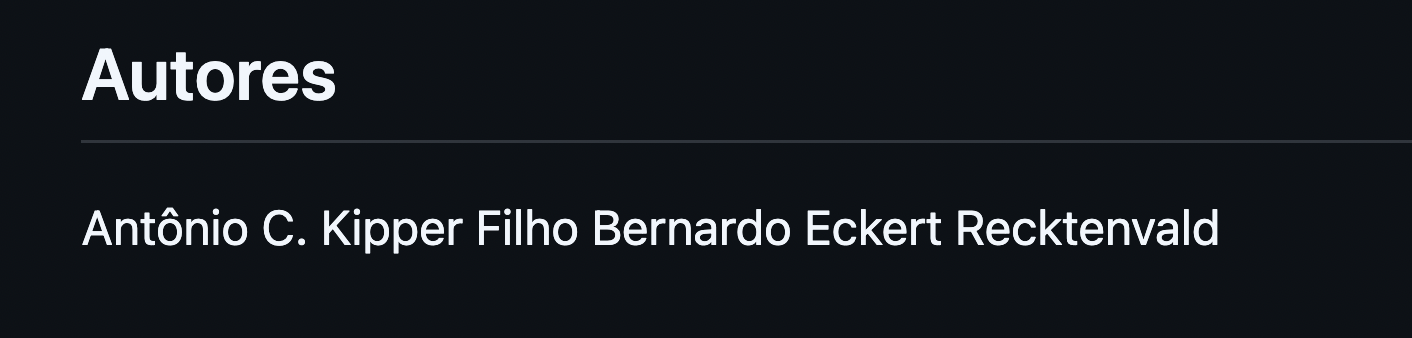
\includegraphics[width=0.6\textwidth]{imgs/tutorial_contribuicao/README_antes_modif.png}
        \caption{README com erro de formatação.}
        \label{fig:README_antes_modif}
    \end{figure}

        \item Na sequência, foram feitas as seguintes modificações:

        \begin{figure}[H]
        \centering
        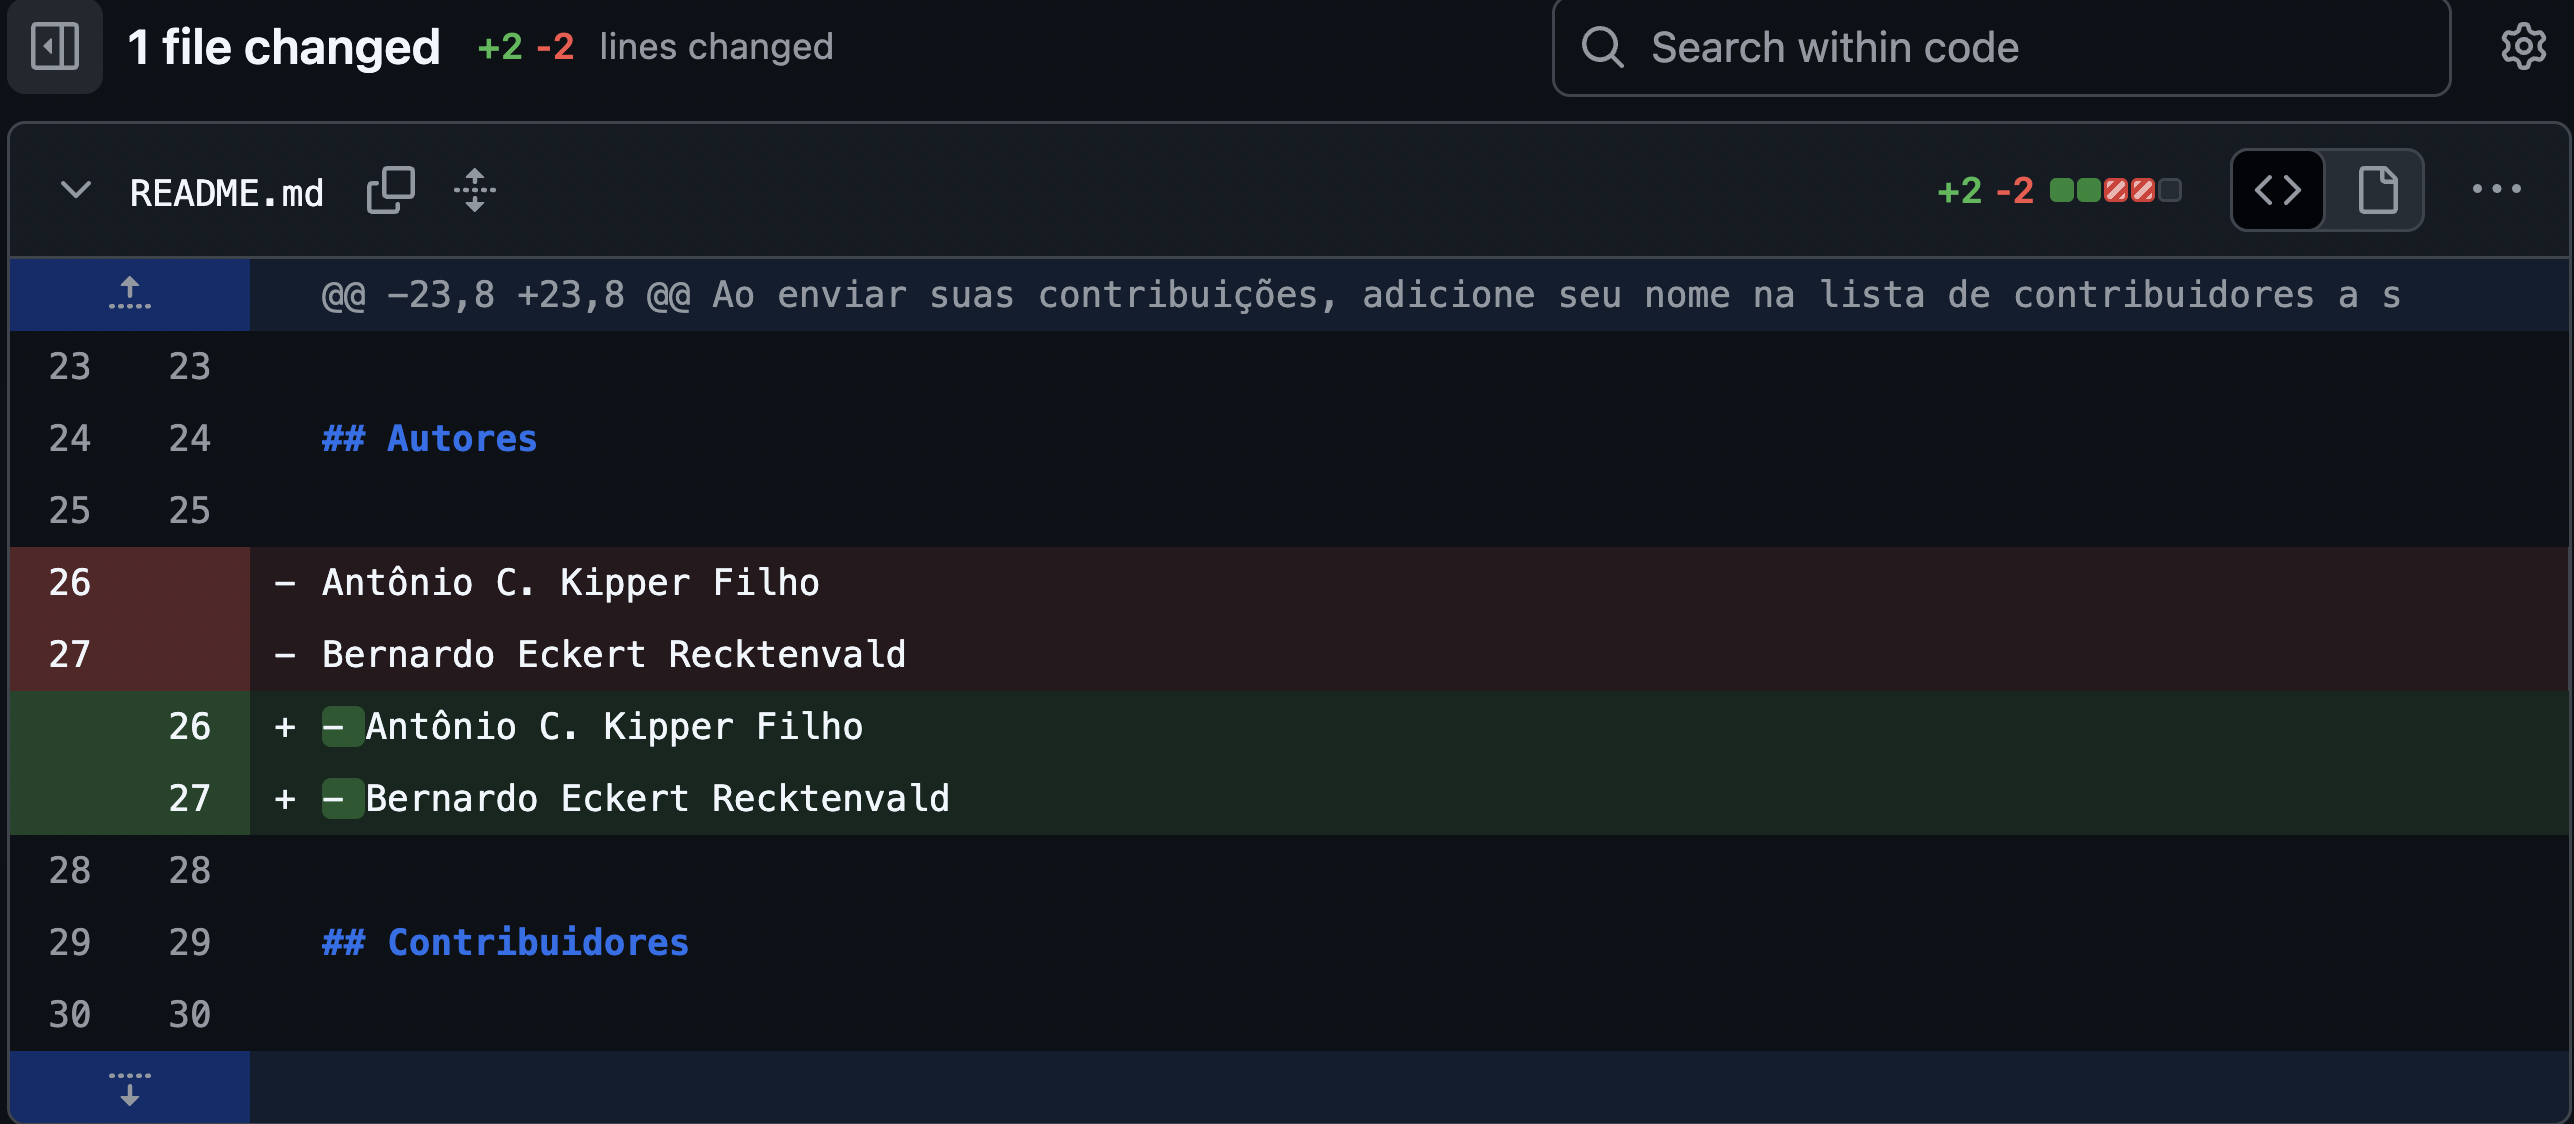
\includegraphics[width=0.6\textwidth]{imgs/tutorial_contribuicao/README_modif.png}
        \caption{Modificações no README - adicionar "-" antes de cada nome para exibição correta como item.}
        \label{fig:README_modif}
    \end{figure}

        \item O resultado esperado é este:

        \begin{figure}[H]
        \centering
        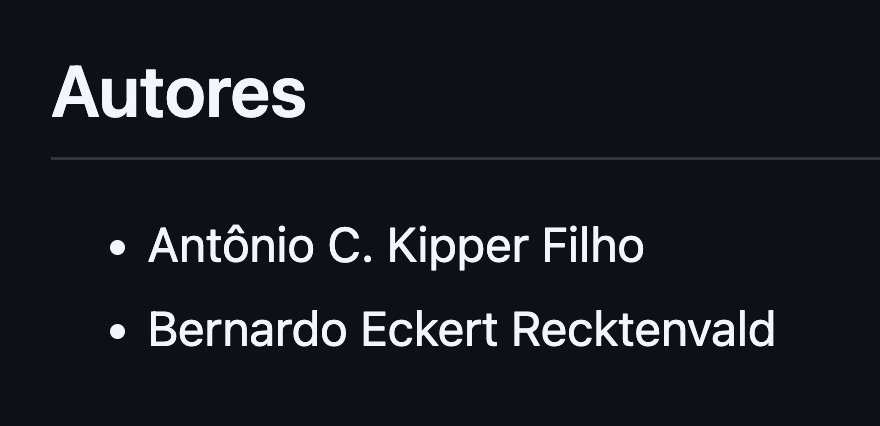
\includegraphics[width=0.6\textwidth]{imgs/tutorial_contribuicao/README_depois_modif.png}
        \caption{README corrigido.}
        \label{fig:README_depois_modif}
    \end{figure}

        \item Adicione, faça commit e envie para seu repositório:
        \begin{lstlisting}[style=shellstyle]
git add .
git commit -m "Descreva sua contribuição"
git push origin minha-contribuicao
        \end{lstlisting}

        \item Na sequência, abra novamente o seu repositório no Github e navegue para a branch de contribuições:

         \begin{figure}[H]
        \centering
        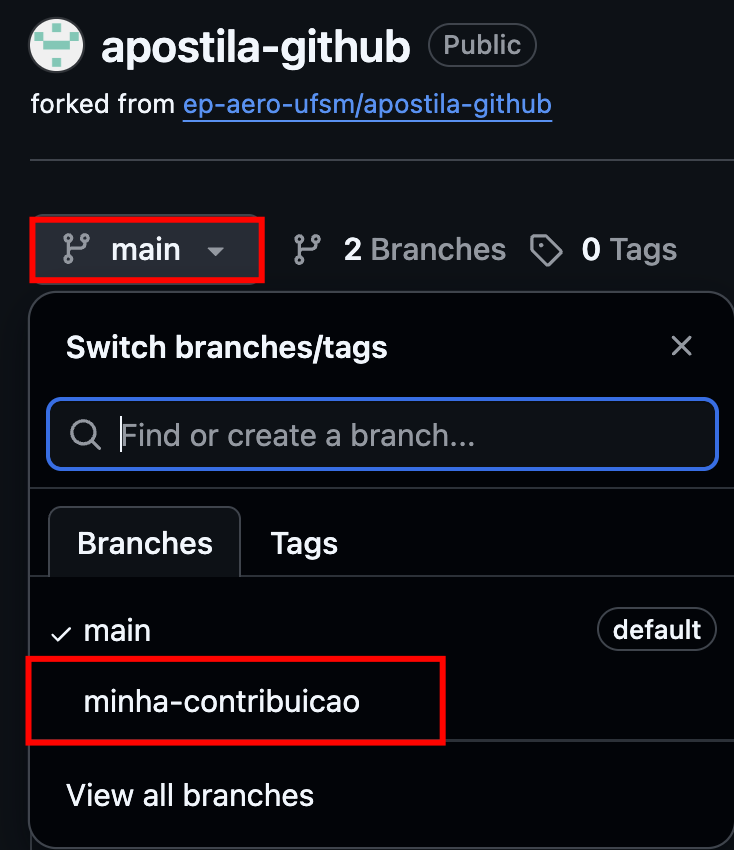
\includegraphics[width=0.6\textwidth]{imgs/tutorial_contribuicao/navegando_branch.png}
        \caption{Navegue para a branch minha-contribuicao.}
        \label{fig:navegando_branch}
    \end{figure}

        \item Abra um Pull Request no repositório original da EP Aero pelo Github. Para fazer isso, siga os passos a seguir:

    \begin{figure}[H]
        \centering
        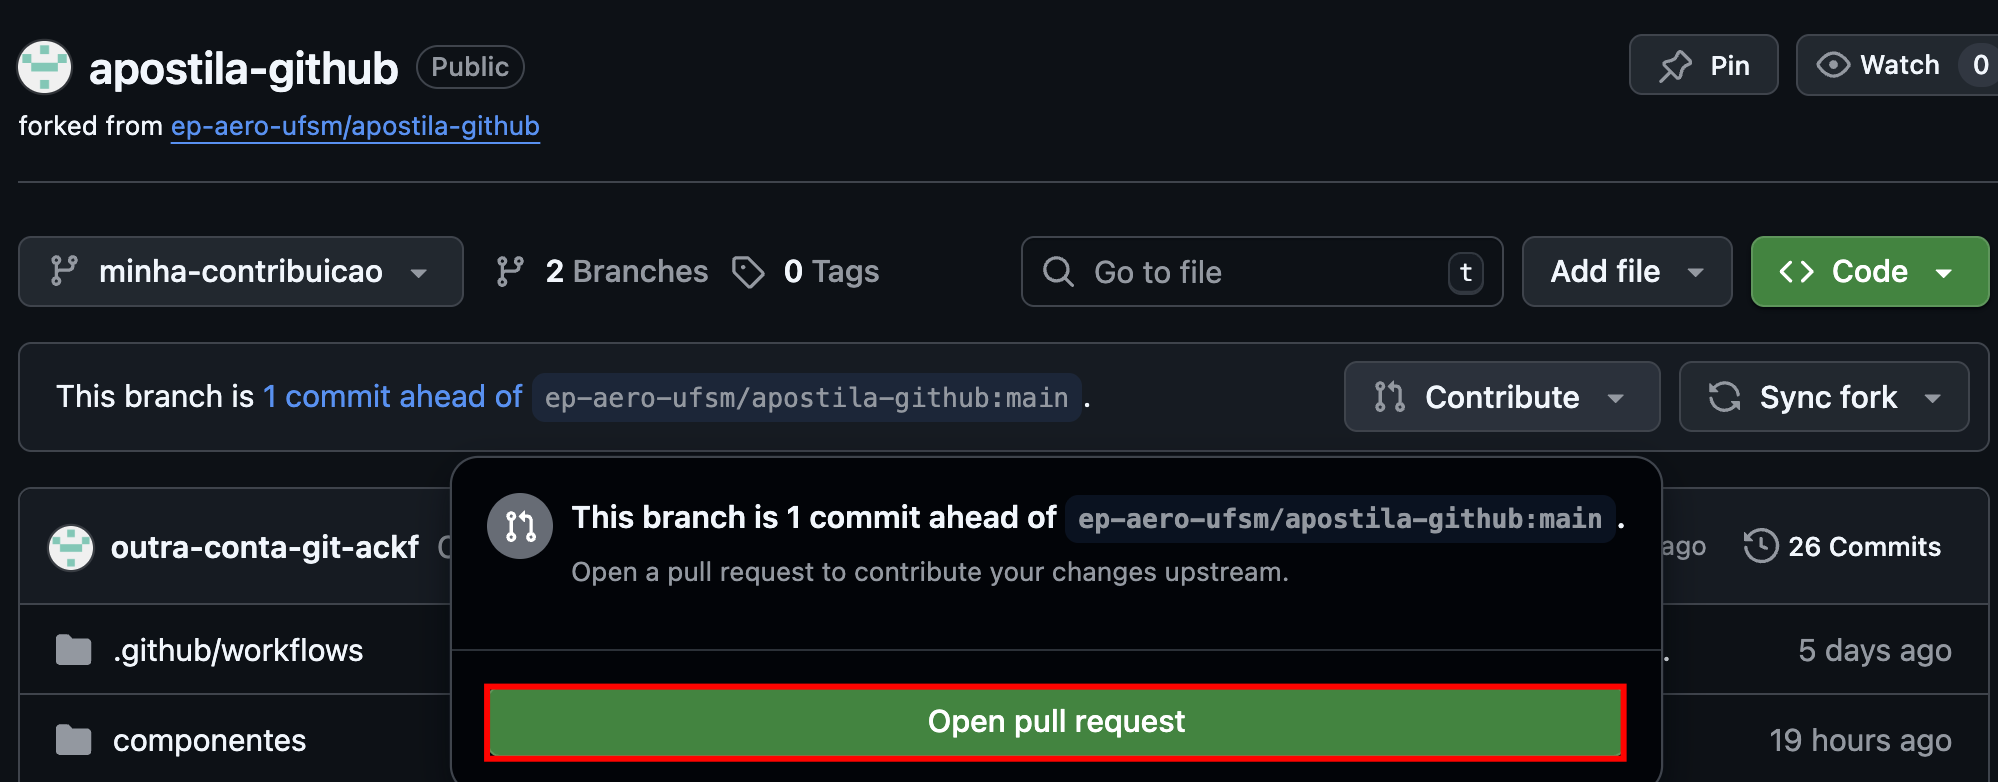
\includegraphics[width=0.6\textwidth]{imgs/tutorial_contribuicao/abrir_pull_request.png}
        \caption{Abra um pull request na sua branch.}
        \label{fig:abrir_pr}
    \end{figure}

    \begin{figure}[H]
        \centering
        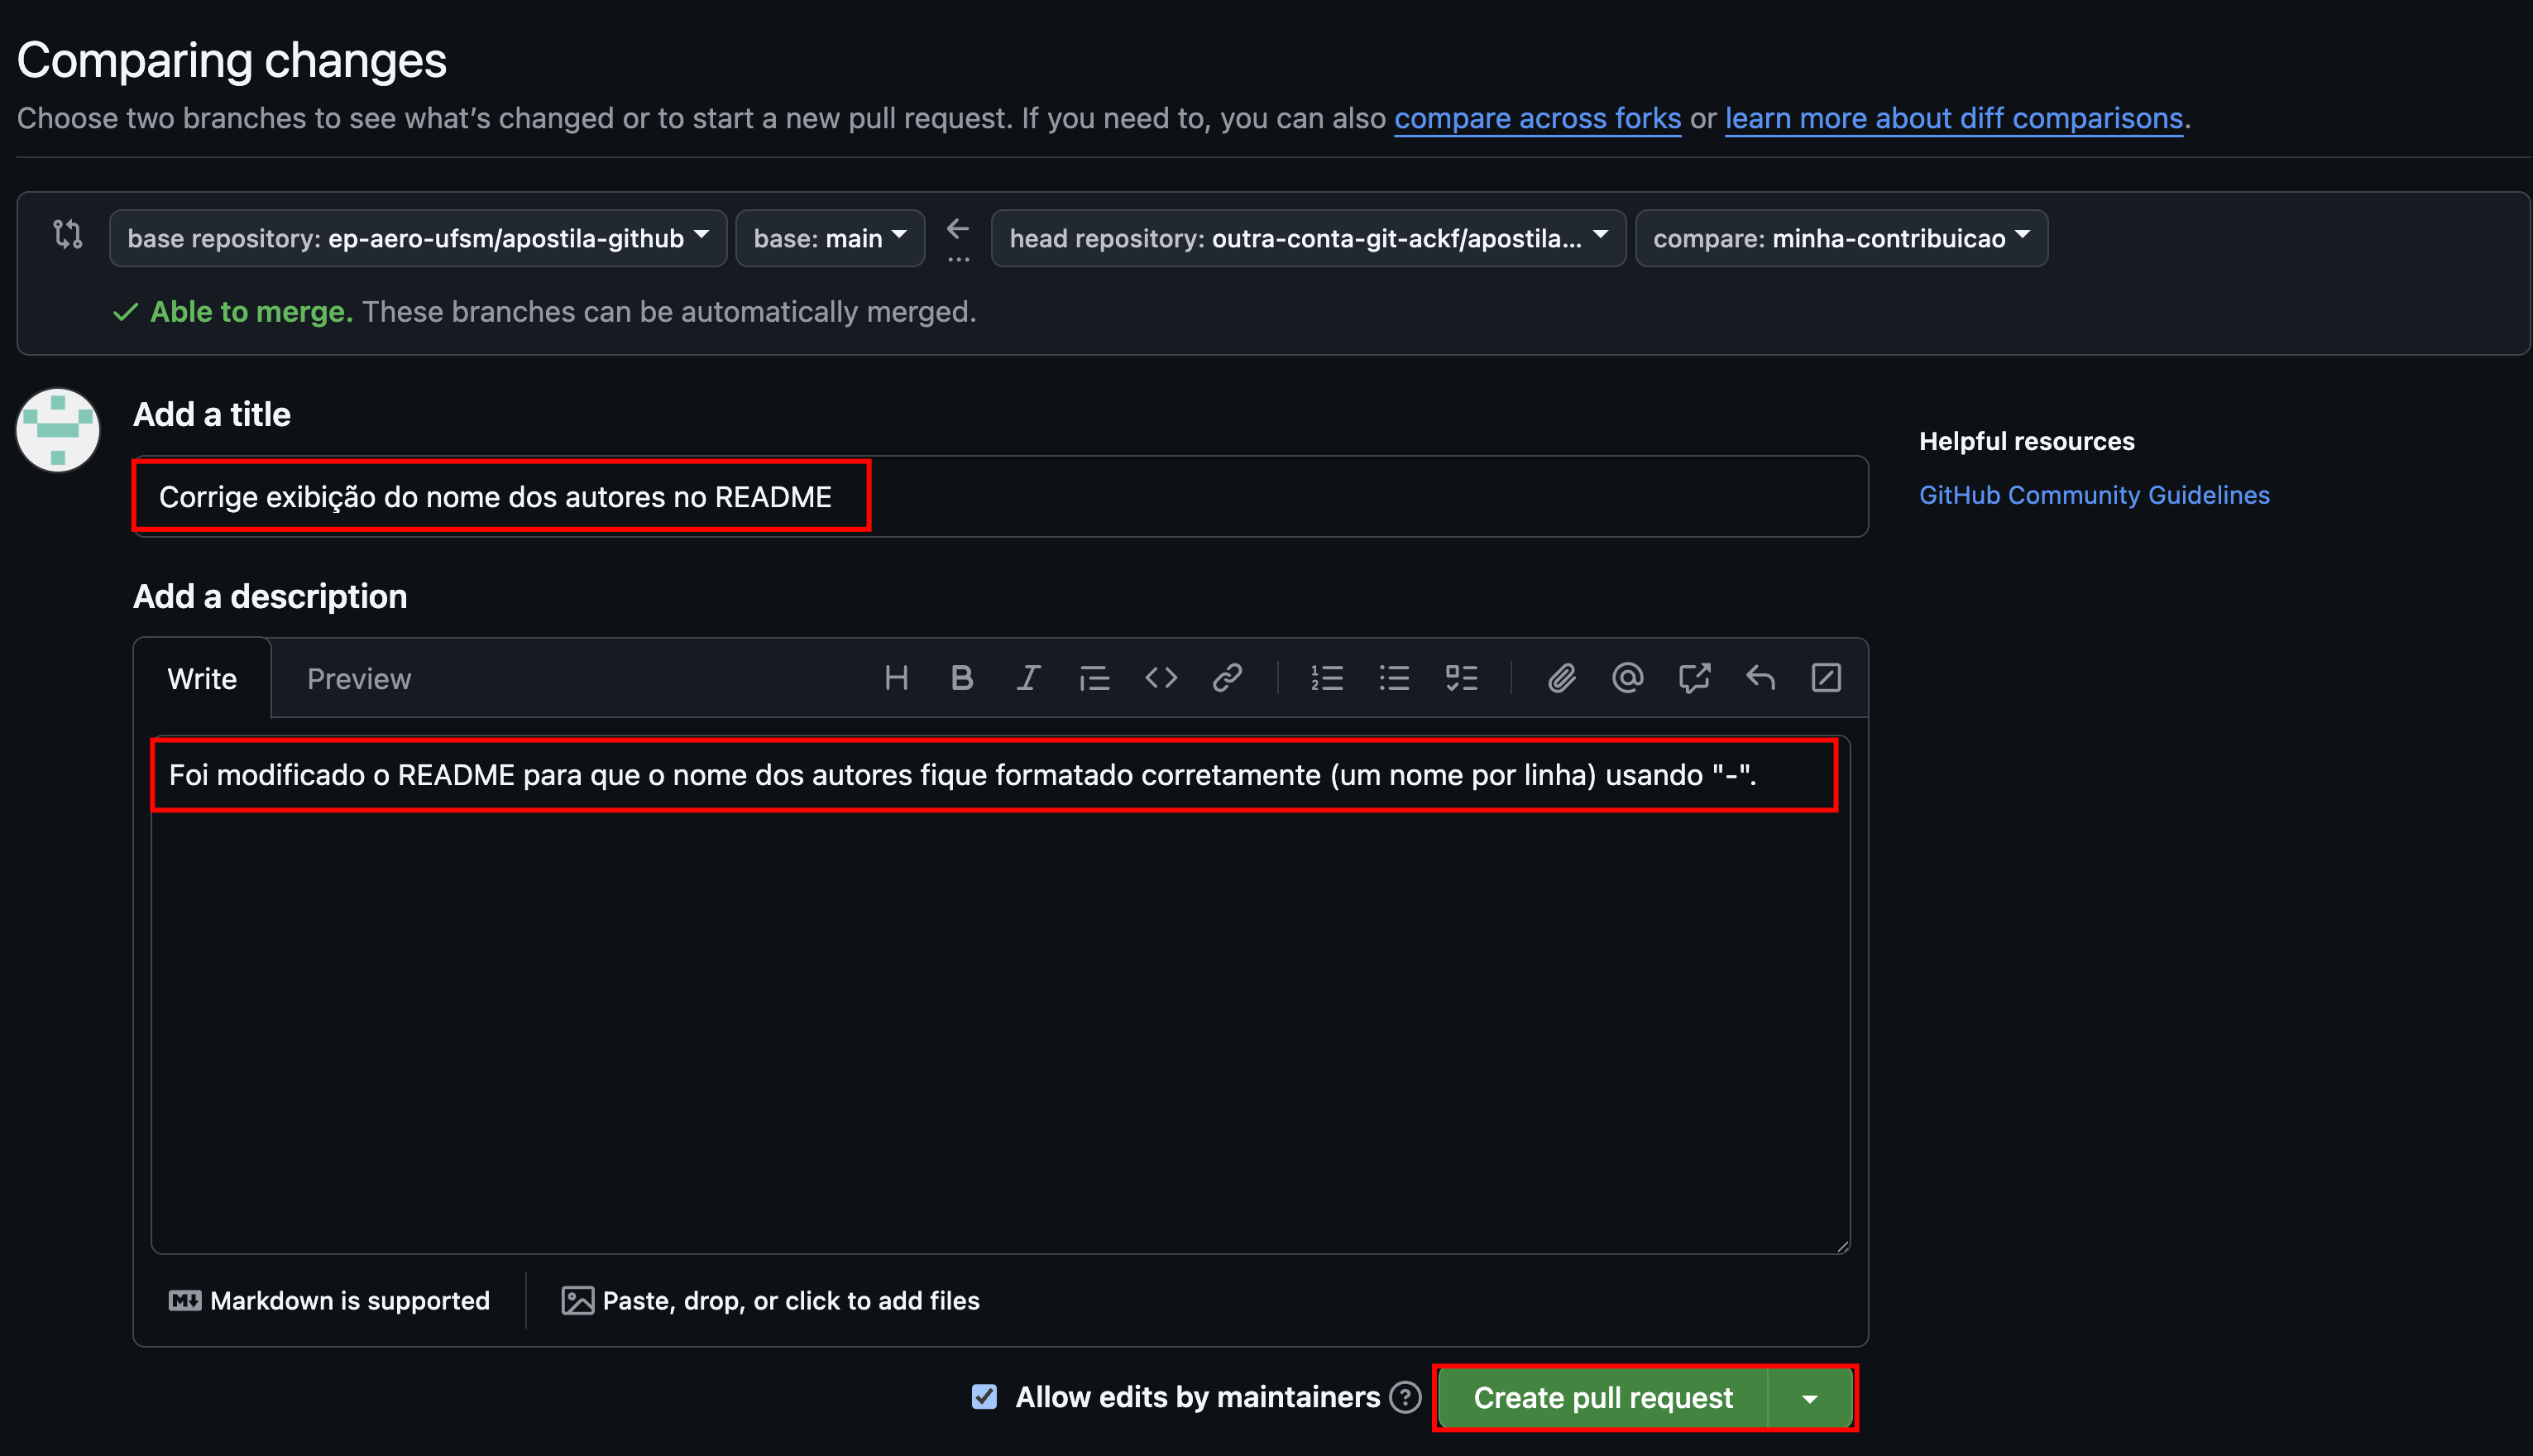
\includegraphics[width=0.6\textwidth]{imgs/tutorial_contribuicao/configurando_pull_request.png}
        \caption{Descreva o pull request. Use um título e uma descrição concisa, mas precisa.}
        \label{fig:configurar_pr}
    \end{figure}

    \item Na sequência, um dos mantedores do repositório da EP Aero UFSM irá analisar seu pull request, e poderá ou aceitá-lo diretamente, ou rejeitá-lo pedindo algum tipo de correção. Caso esse seja o caso, você receberá uma mensagem como esta no seu pull request:

    \begin{figure}[H]
        \centering
        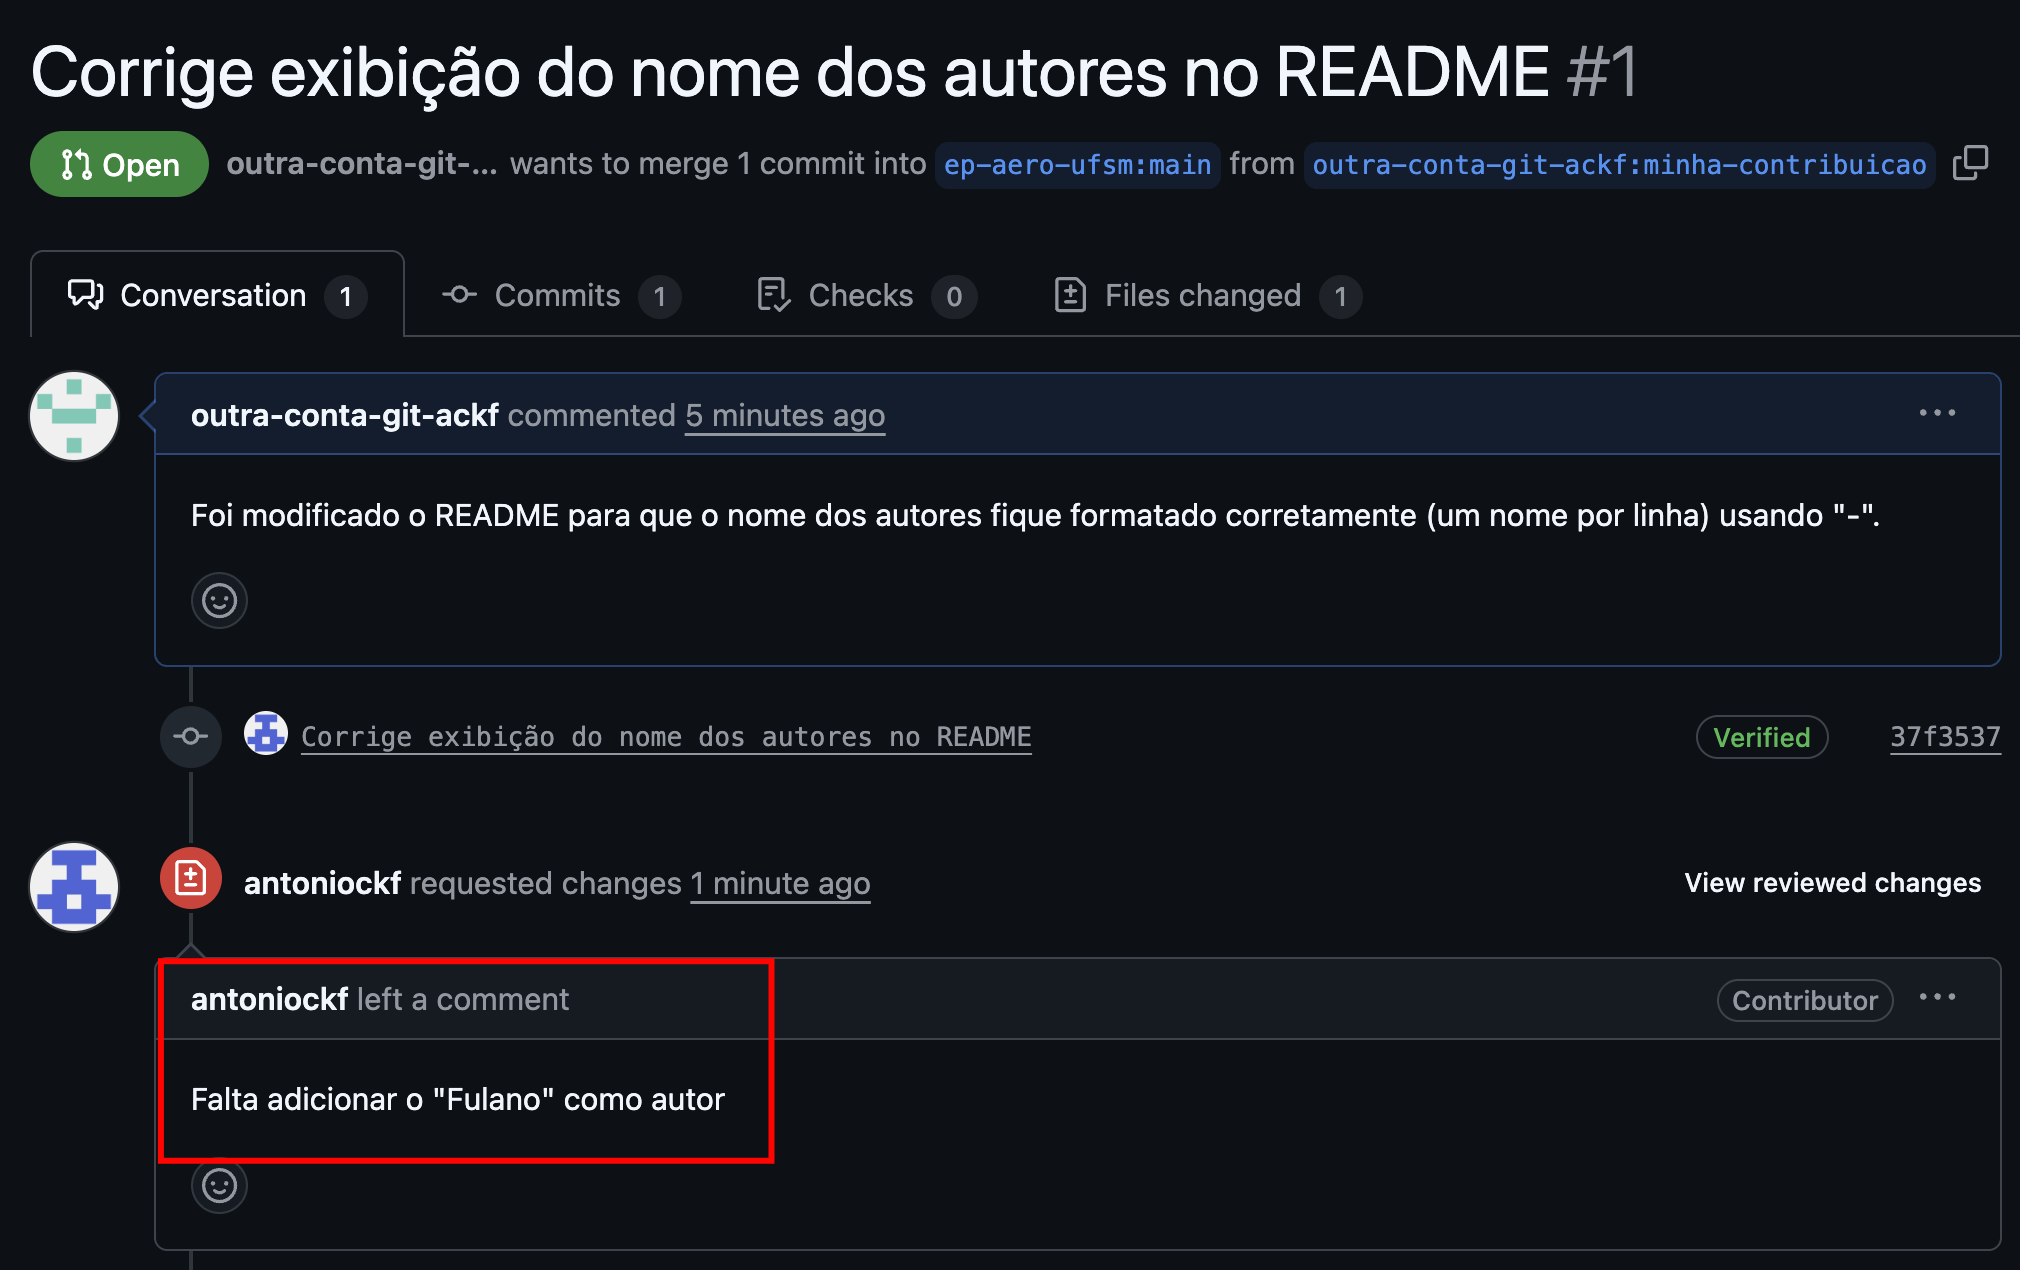
\includegraphics[width=0.6\textwidth]{imgs/tutorial_contribuicao/pr_rejeitado.png}
        \caption{Pull request rejeitado - os mantedores solicitam modificações.}
        \label{fig:pr_rejeitado}
    \end{figure}

    \item Você deve então fazer um novo commit na sua branch com as correções pedidas. O novo commit aparecerá automaticamente no Pull Request que você havia enviado antes:

    \begin{figure}[H]
        \centering
        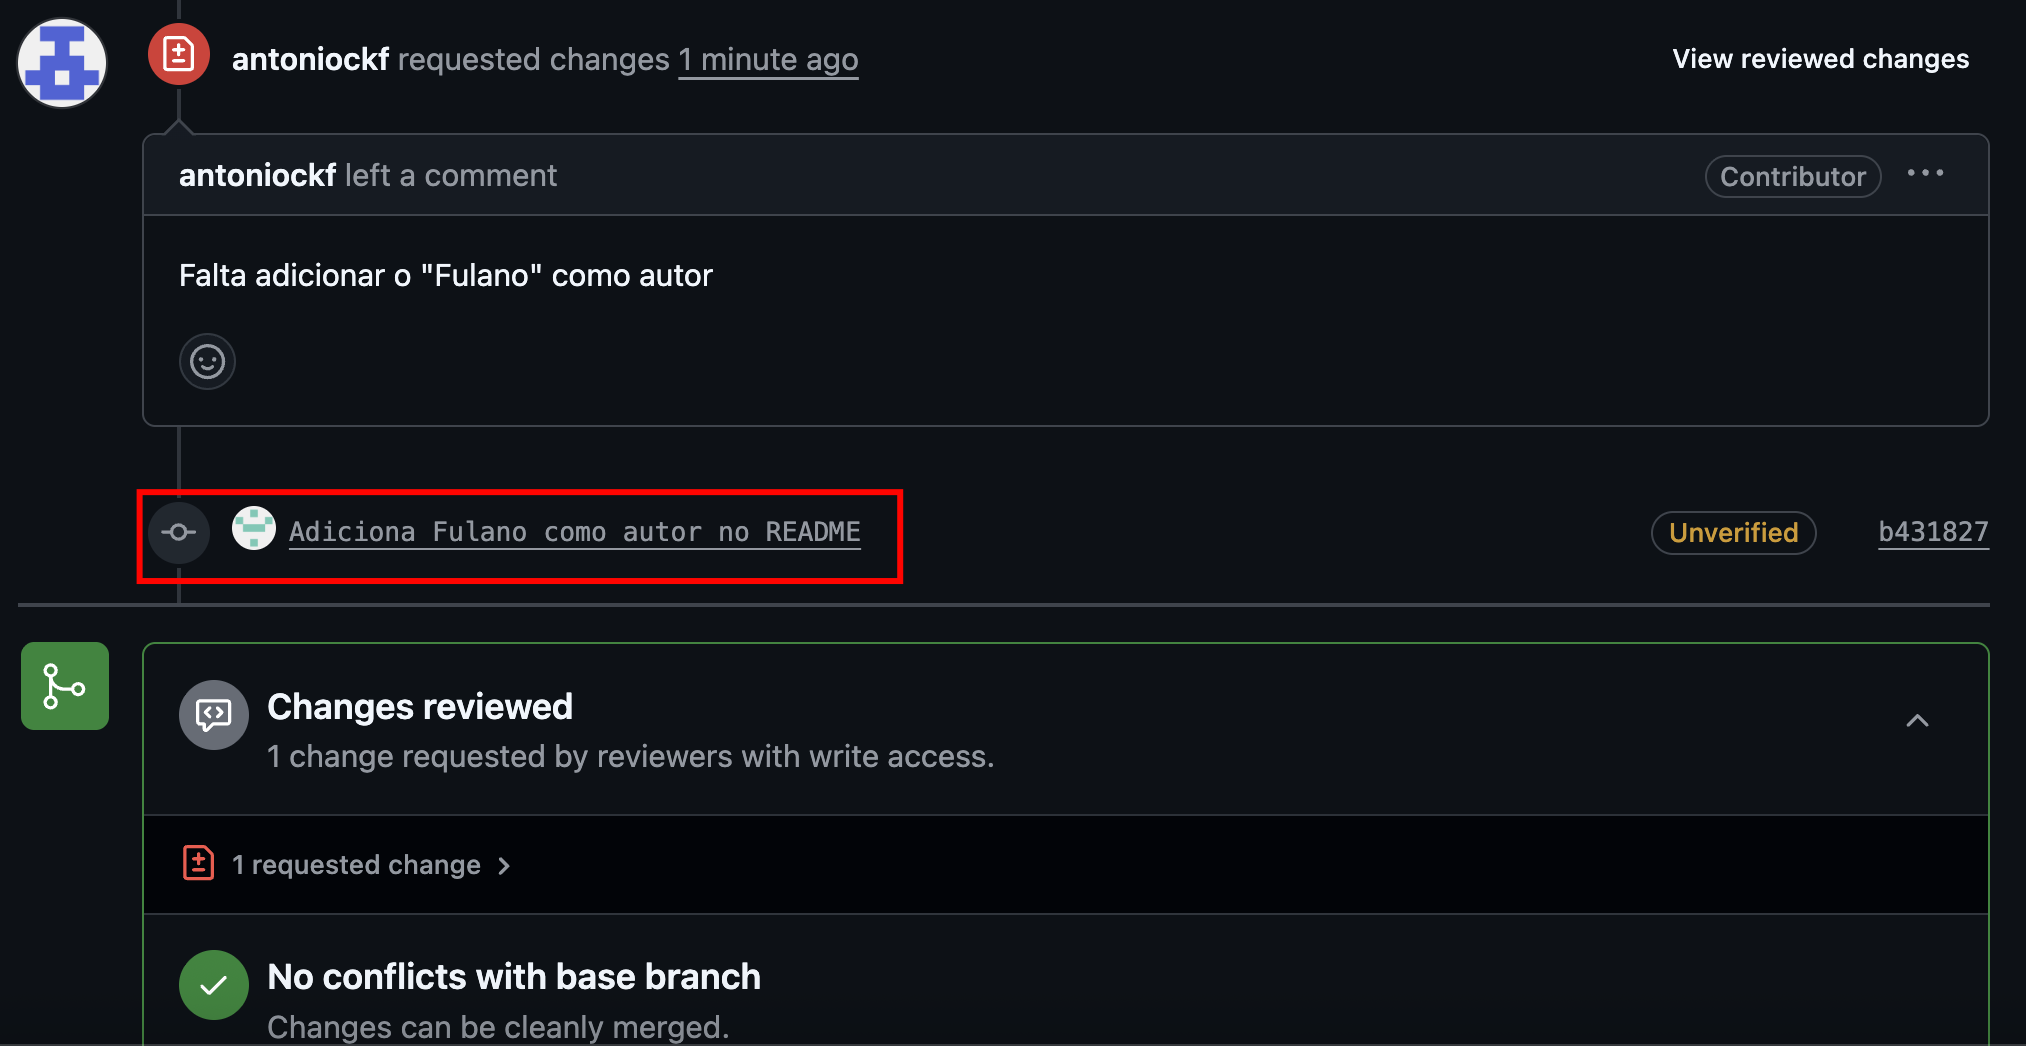
\includegraphics[width=0.6\textwidth]{imgs/tutorial_contribuicao/replica_pr.png}
        \caption{Mudança no PR após solicitação de correção.}
        \label{fig:replica_pr}
    \end{figure}

    \item Quando o PR for aceito, ele aparecerá na história de commits da branch principal do repositório da EP Aero: 

    \begin{figure}[H]
        \centering
        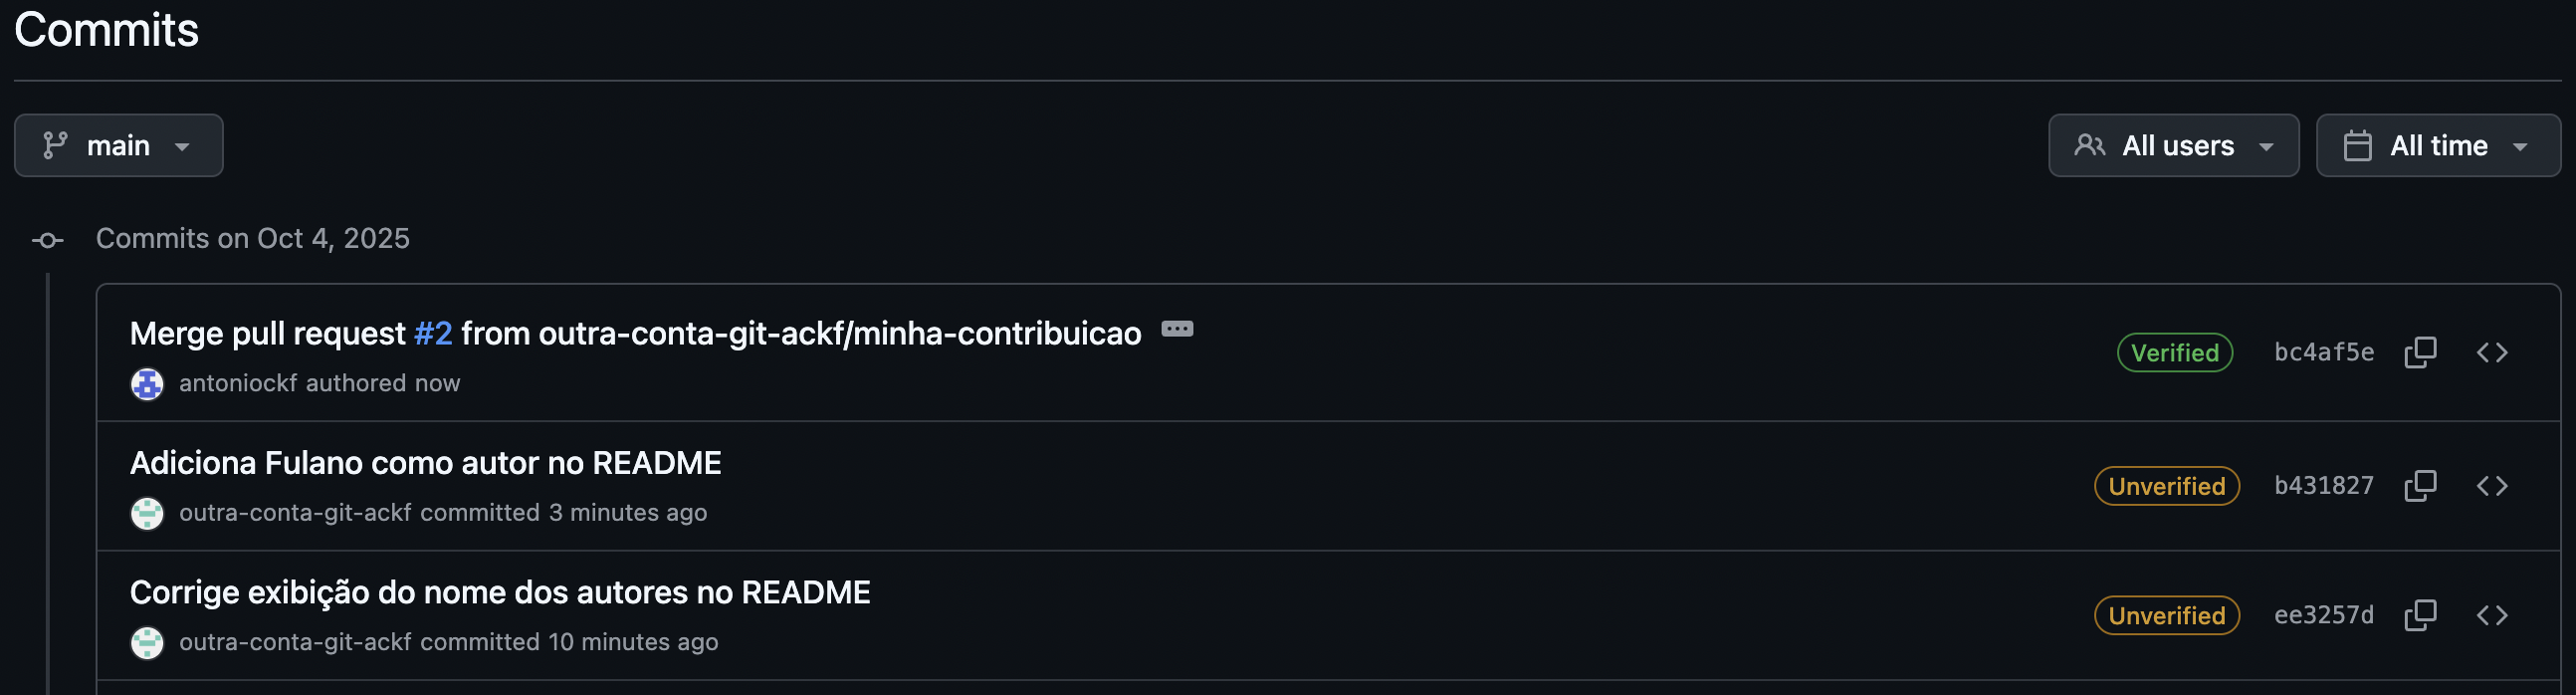
\includegraphics[width=0.6\textwidth]{imgs/tutorial_contribuicao/resultado_pr.png}
        \caption{Resultado final após merge do PR.}
        \label{fig:resultado_pr}
    \end{figure}
\end{itemize}